\documentclass[12pt,a4paper]{article}

\usepackage{amsfonts}
\usepackage{amssymb}
\usepackage{amsmath}
\usepackage{amsthm}
\usepackage{epsfig}
\usepackage{graphicx}
\usepackage{natbib}		% citet, citep
\usepackage{textcomp}
\usepackage{booktabs}
\usepackage{multirow}
\usepackage{fullpage}
\usepackage{authblk}
\usepackage{url}
\usepackage{color}
\usepackage{float}
\usepackage{enumitem}

\begin{document}

\subsection*{I. Algorithm Design}

To solve the car rental scheduling problem across varying scales and ensure the program generates a feasible solution within the 3-minute limit, our algorithm adopts a \textbf{Three-Tier Adaptive Architecture}.

The key idea behind our design is to use different strategies for different instance sizes. Small instances are solved using a Path-flow Mixed-Integer Programming (MIP) model, medium-sized instances are handled by a Revenue-first Insertion Heuristic, and large instances are solved by a fast Heap-Based Chronological Greedy approach. This design allows us to achieve a good balance between solution quality and computational efficiency.

\subsection*{II. Algorithm Structure}

\subsection*{1. Flow Chart}
\begin{figure}[H]
    \centering
    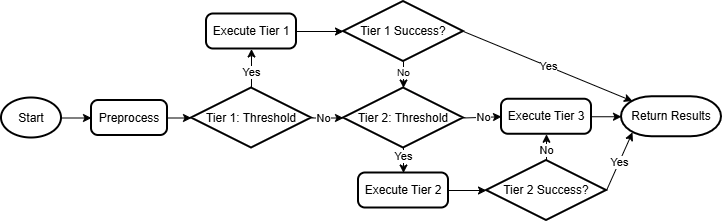
\includegraphics[width=0.9\linewidth]{OR_flowchart.png}
\end{figure}

\subsection*{2. Data Preprocessing and Optimization}
\begin{itemize}
    \item \textbf{Time Cache:} Converts all string-formatted times into ``minutes elapsed since 2023/1/1 00:00.'' It establishes a cache using a Dictionary to avoid massive repeated string parsing, significantly reducing the I/O conversion burden.
    \item \textbf{Matrix for Moving Times:} Creates a 2D array \texttt{moving\_time[i][j]}, allowing all queries for moving times between stations to be completed in $\mathcal{O}(1)$ time.
\end{itemize}

\subsection*{3. Tier 1: Small Instances (Path-flow MIP)}
\begin{itemize}
    \item \textbf{Trigger Condition:} $K \le 160$ and $C \cdot K^2 \le 700000$.
    \item \textbf{Logic:} Transforms the problem into a network flow model in graph theory. It uses decision variables $x_{c,i,j}$ to determine whether car $c$, after serving order $i$, has sufficient cleaning and moving time to consecutively serve order $j$. The Gurobi time limit is set to 20 seconds; if solved successfully, it directly returns the optimized schedule.
\end{itemize}

\subsection*{4. Tier 2: Medium Instances (Revenue-first Insertion Heuristic)}
\begin{itemize}
    \item \textbf{Trigger Condition:} $K \le 6000$ and $C \cdot K \le 600000$.
    \item \textbf{Logic:} Driven by the intuition of ``maximizing business profit.''
    \begin{enumerate}[label=\textbf{\alph*.}]
        \item Sorts all orders in descending order based on Revenue.
        \item Processes high-revenue orders first, searching for candidate cars that meet the level constraints (same level or free upgrade).
        \item Utilizes Binary Search to attempt inserting the new order into the car's existing schedule (sorted by pick-up time).
        \item Checks the ``previous'' and ``next'' orders at the insertion position to ensure no scheduling conflicts occur after adding cleaning and moving times. Assigns the car that consumes the least additional relocation budget.
    \end{enumerate}
\end{itemize}

\subsection*{5. Tier 3: Large Instances (Heap-Based Chronological Greedy)}
\begin{itemize}
    \item \textbf{Trigger Condition:} The ultimate fallback plan when the first two tiers time out or the instance size is too large.
    \item \textbf{Logic:} Simulates the passage of time in the real world.
    \begin{enumerate}[label=\textbf{\alph*.}]
        \item Creates a Min-Heap for each station and each car level, using the car's ``earliest ready time'' as the sorting criterion.
        \item Sorts the orders chronologically by Pickup Time.
        \item As time advances to a specific order, it prioritizes extracting the earliest ready car from the pick-up station's Heap at a speed of $\mathcal{O}(\log C)$.
        \item If no cars are available locally, it scans a pre-built ``Nearest Stations list,'' evaluates the moving time and remaining budget, and relocates a car from a nearby station. After completing the order, it updates the car's Ready Time and pushes it into the drop-off station's Heap.
    \end{enumerate}
\end{itemize}

\subsection*{III. Time Complexity}

The following variables are defined: $K$ as the number of orders, $C$ as the total number of cars, $S$ as the number of stations, and $L$ as the number of car levels.

\subsection*{1. Data Preprocessing}
Reading data and establishing foundational arrays, including $\mathcal{O}(S^2)$ to build the moving time matrix and $\mathcal{O}(K)$ to convert order times. Preprocessing Complexity:
$$ T_{\text{preprocessing}} = \mathcal{O}(K + C + S^2) $$

\subsection*{2. MIP}
The main loop for Arc creation is $\mathcal{O}(n_C \cdot n_K^2)$, therefore:
$$T_{\text{MIP}} = \mathcal{O}(n_C \cdot n_K^2)$$

\subsection*{3. Insertion Heuristic}
\begin{itemize}
    \item Sort orders: $\mathcal{O}(n_K \log n_K)$
    \item For each order, scan all candidate cars and perform binary search: $\mathcal{O}(n_C \log n_K)$
    \item Actual insert operation: $\mathcal{O}(n_K)$ per insertion
    \item Total complexity:
    $$T_{\text{insertion}} = \mathcal{O}(n_K \cdot n_C \cdot \log n_K + n_K^2)$$
\end{itemize}

\subsection*{4. Heap-Based Greedy}
\begin{itemize}
    \item Precompute nearest neighbor list: $\mathcal{O}(n_S^2 \log n_S)$
    \item Sort orders: $\mathcal{O}(n_K \log n_K)$
    \item Process each order: Local station check $\mathcal{O}(n_L)$, Cross-station scan $\mathcal{O}(\text{scan\_limit} \cdot n_L \cdot \log n_C)$
    \item Total complexity (Large $n_S$ scenario):
    $$T_{\text{greedy}} = \mathcal{O}(n_S^2 \log n_S + n_K \cdot \sqrt{n_S} \cdot n_L \cdot \log n_C)$$
\end{itemize}

\end{document}
